\documentclass{beamer}
%\usepackage{beamerthemeAmsterdam}
\usepackage{amsmath}
\usepackage{graphicx}

\usepackage{color}
\usepackage{hyperref}
\hypersetup{linkcolor=blue,filecolor=red}

\title{JPEG-2000}
\subtitle{De Wondere Wereld van Wavelets}
\author{Jan Westerdiep \and Okke van Garderen}
\date{\today}
\institute{Universiteit van Amsterdam}

\begin{document}

\frame{\titlepage}

\section{Intro}
\frame{
  \frametitle{Vakantieplaatje}
  \begin{columns}
    \begin{column}{0.5\textwidth}
      \hfill
      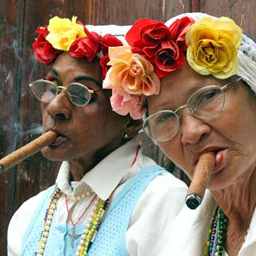
\includegraphics[width=\textwidth]{cigar.png}
      \hfill
    \end{column}
    \pause
    \begin{column}{0.5\textwidth}
      \hfill
      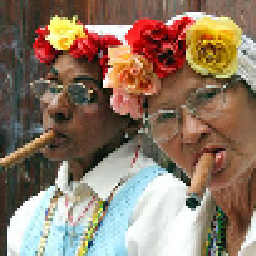
\includegraphics[width=\textwidth]{cigar_downscale.png}
      \hfill
    \end{column}
  \end{columns}
}
\frame{
  \frametitle{Vakantieplaatje}
  \begin{columns}
    \begin{column}{0.5\textwidth}
      \hfill
      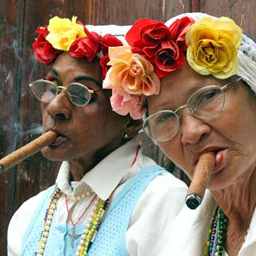
\includegraphics[width=\textwidth]{cigar.png}
      \hfill
    \end{column}
    \begin{column}{0.5\textwidth}
      \hfill
      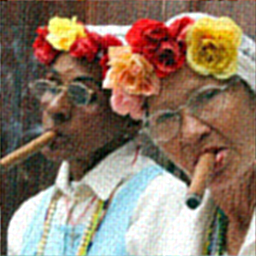
\includegraphics[width=\textwidth]{cigar_fourier.png}
      \hfill
    \end{column}
  \end{columns}
}
\frame{
  \frametitle{Vakantieplaatje}
  \begin{columns}
    \begin{column}{0.5\textwidth}
      \hfill
      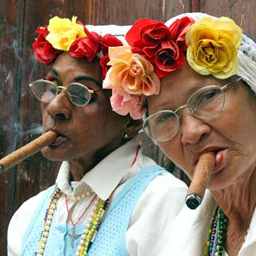
\includegraphics[width=\textwidth]{cigar.png}
      \hfill
    \end{column}
    \begin{column}{0.5\textwidth}
      \hfill
      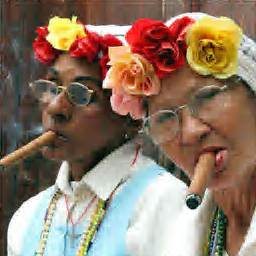
\includegraphics[width=\textwidth]{cigar_db2.png}
      \hfill
    \end{column}
  \end{columns}
}

\frame{
	\frametitle{Ons project}
	\begin{itemize}
		\item Beeldcompressie
		\item JPEG: Fouriertransformatie
		\item JPEG-2000: Wavelettransformatie
	\end{itemize}
}

\frame{
	\frametitle{Fouriertransformatie}
	\begin{itemize}
	\item Beginsignaal $f$
	\item Transformatie is omschrijven naar andere basis 
          \[
          f = \sum_k \langle f,\phi_k \rangle \phi_k
          \]
          \vspace{-15pt}
        \item Fourier:
          \[ \phi_k(n) = e^{2\pi i k n /N} = \cos(2\pi kn/N) + i\cdot\sin(2\pi kn/N)\]
          \vspace{-15pt}
	  \begin{itemize}
	  \item Voorbeeld: $\pi$ schrijven in termen van machten van tien (decimale ontwikkeling)
	  \end{itemize}
	\item Compressie door minst significante termen weg te laten
	  \begin{itemize}
	  \item $\pi \simeq 3.1415$ is `wel precies genoeg'
	  \end{itemize}
	\item Nadeel: werkt niet goed bij plaatjes met scherpe randen
	\end{itemize}
}

\frame{
	\frametitle{Wavelettransformatie}
	\begin{columns}
		\begin{column}{0.5\textwidth}
			\begin{itemize}
				\item Weer omschrijven in een andere basis
				\item Heel veel soorten wavelets
				\item (Wiskundig wat interessanter: relatief nieuw)
				\item Inzichtelijker -> als in de transform ziet er duidelijk uit (geeft ons weer reden tot een plaatje)
			\end{itemize}
		\end{column}
		\begin{column}{0.5\textwidth}
			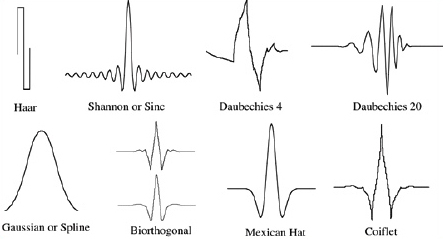
\includegraphics[width=\textwidth]{wavelets.jpg}\\
			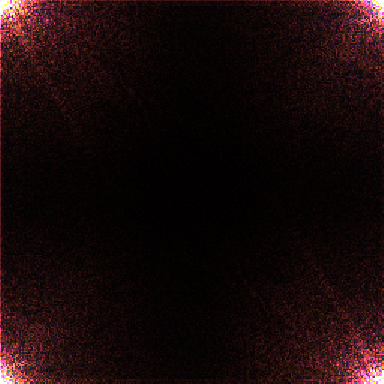
\includegraphics[width=0.5\textwidth]{cigar_transform_fourier.pdf}
			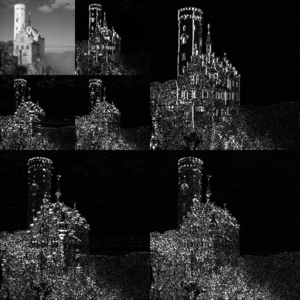
\includegraphics[width=0.5\textwidth]{huis_wavelet_transformed.png}
		\end{column}
	\end{columns}
}

\frame{
	\frametitle{Voorbeelden (1\%)}
  \begin{table}
    \begin{tabular}{c c c c}
      Downscale &
      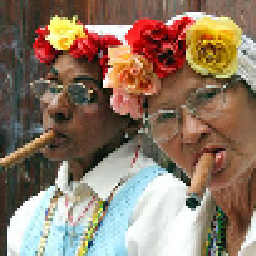
\includegraphics[width=0.3\linewidth]{cigar_downscale.png} &
      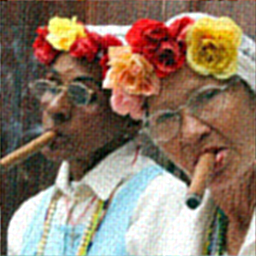
\includegraphics[width=0.3\linewidth]{cigar_fourier.png} &
      Fourier \\
      Haar &
      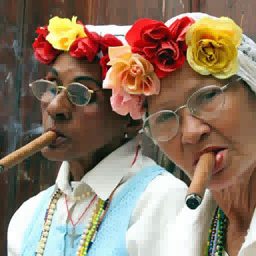
\includegraphics[width=0.3\linewidth]{cigar_haar.png} &
      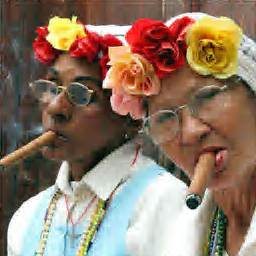
\includegraphics[width=0.3\linewidth]{cigar_db2.png} &
      Daubechies 2
    \end{tabular}
  \end{table}
}

\frame{
	\frametitle{Filmpjes (0.2\%)}
        \href{pag6b.html}{Link naar gifjes}
        
}
\end{document}
